\documentclass{../class/tae-ufla-article}
\usepackage[utf8]{inputenc}

\usepackage{lipsum}
\usepackage{graphicx}
\addbibresource{myreferences.bib}

\begin{document}




\twocolumn[{%
\teatitleformat{A very large title created only to test the spacing behavior}
\taeauthorformat{John Doe}{Biology Deparmento of UFLA}
\taeauthorformat{Jane Doe}{Biology Deparmento of UFLA}
%\taeauthorformat{\lipsum[1]}{\lipsum[1]}
\begin{teaabstract}
\lipsum[1]
\end{teaabstract}
\begin{teakeywords}
palavra1, palavra2, palavra3, palavra4.
\end{teakeywords}
\begin{teadata}
Received: November 07, 2022 - Accepted: March 03, 2023
\end{teadata}
}]
\thispagestyle{empty}
\fontsize{11pt}{14pt}\selectfont

\renewcommand{\taefoottext}{THEORETICAL AND APPLIED ENGINEERING - UFLA - LAVRAS - V7 - N1 - 2023 - P. 1-8}
\renewcommand{\taeheadoddtext}{MULTISENSOR ANALYSIS IN A TEAK REFORESTATION AREA IN THE LEGAL AMAZON, BRAZIL}
\renewcommand{\taeheadeventext}{TRINDADE, L. R. S. L. C. et al.}
%%%%%%%%%%%%%%%%%%%%%%%%%%%%%%%%%%%%%%%%%%%%%%%%%%%%%%%%%%%%%%%%%%%%%%%%%%%%%%%%%%%%%%%%%%%%%%%%%
\section{A very large title section name}

\lipsum[1-2]
\begin{figure}[!ht]
  \centering
  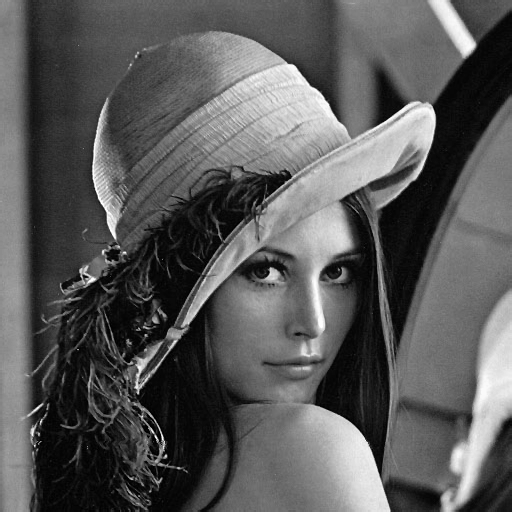
\includegraphics[width=0.25\textwidth]{screenshot.png}
  \caption{A picture of Lena}
\end{figure}
\lipsum[1]. See the Eq. \ref{eq:1} or \ref{eq:2}
\begin{equation}\label{eq:1}
x=\sum_{n}^{N}a^{n}
\end{equation}
\lipsum[1] $x+y+z=0$ some text $x=\sum_{n}^{N}a^{n}$ \lipsum[1] 
\begin{equation}\label{eq:2}
y=\sum_{n}^{N}b^{n}
\end{equation}

%%%%%%%%%%%%%%%%%%%%%%%%%%%%%%%%%%%%%%%%%%%%%%%%%%%%%%%%%%%%%%%%%%%%%%%%%%%%%%%%%%%%%%%%%%%%%%%%%
\section{Title of section}
\lipsum[1] 
Table \ref{table:1} is an example of a referenced \LaTeX{} element.

\begin{table}[h!]
\centering
\caption{Table to test captions and labels.}
\label{table:1}
\begin{tabular}{||c c c c||} 
 \hline
 Col1 & Col2 & Col2 & Col3 \\ [0.5ex] 
 \hline\hline
 1 & 6 & 87837 & 787 \\ 
 2 & 7 & 78 & 5415 \\
 3 & 545 & 778 & 7507 \\
 4 & 545 & 18744 & 7560 \\
 5 & 88 & 788 & 6344 \\ [1ex] 
 \hline
\end{tabular}
\end{table}
\lipsum[1]

%%%%%%%%%%%%%%%%%%%%%%%%%%%%%%%%%%%%%%%%%%%%%%%%%%%%%%%%%%%%%%%%%%%%%%%%%%%%%%%%%%%%%%%%%%%%%%%%%
\section{Conclusion}
\lipsum[1] \cite{texbook} \cite{latex:companion}


%%%%%%%%%%%%%%%%%%%%%%%%%%%%%%%%%%%%%%%%%%%%%%%%%%%%%%%%%%%%%%%%%%%%%%%%%%%%%%%%%%%%%%%%%%%%%%%%%


\printbibliography[title=References]

\end{document}














